\documentclass{article}


% if you need to pass options to natbib, use, e.g.:
%     \PassOptionsToPackage{numbers, compress}{natbib}
% before loading neurips_2023


% ready for submission
\usepackage[nonatbib, final]{neurips_2020}
\usepackage{subcaption}

\usepackage[utf8]{inputenc}
\usepackage{hyperref}
\usepackage{graphicx}
\usepackage[final]{neurips_2020}
\usepackage{amsmath}
\usepackage{amssymb}
\usepackage[Ink]{svg}


% to compile a preprint version, e.g., for submission to arXiv, add add the
% [preprint] option :
%     \usepackage[preprint]{neurips_2023}


% to compile a camera-ready version, add the [final] option, e.g.:
%     \usepackage[final]{neurips_2023}


% to avoid loading the natbib package, add option nonatbib:
%    \usepackage[nonatbib]{neurips_2023}


\usepackage[utf8]{inputenc} % allow utf-8 input
\usepackage[T1]{fontenc}    % use 8-bit T1 fonts
\usepackage{hyperref}       % hyperlinks
\usepackage{url}            % simple URL typesetting
\usepackage{booktabs}       % professional-quality tables
\usepackage{amsfonts}       % blackboard math symbols
\usepackage{nicefrac}       % compact symbols for 1/2, etc.
\usepackage{microtype}      % microtypography
\usepackage{xcolor}         % colors








\usepackage{verbatim}
\usepackage{stmaryrd}
\usepackage{tikz}
\usetikzlibrary{positioning, arrows.meta}
\usepackage{graphicx}
\usepackage{amsmath}
\usepackage{interval}
\usepackage{bm}


\title{Projet ATIAM 2022-2023 : Exploring the latent space of a temporal VAE for audio loops generation}
\author{Étienne André, Paul Estève, Antoine Souchaud \& Enguérand Tamagna}
%\title{Exploring the latent space of a temporal VAE for audio loops generation}


% The \author macro works with any number of authors. There are two commands
% used to separate the names and addresses of multiple authors: \And and \AND.
%
% Using \And between authors leaves it to LaTeX to determine where to break the
% lines. Using \AND forces a line break at that point. So, if LaTeX puts 3 of 4
% authors names on the first line, and the last on the second line, try using
% \AND instead of \And before the third author name.


%\author{AAAAA}
\usepackage[
backend=biber,
style=numeric,
sorting=ynt
]{biblatex}

\addbibresource{biblio.bib}
% \AtEveryBibitem{%
% \ifentrytype{book,collection,incollection,misc}{
%     \clearfield{url}%
%     \clearfield{urldate}%
%     \clearfield{review}%
%     \clearfield{series}%%
%     \clearfield{primaryclass}
% }{}
% }
% Exclure le champ primaryclass
\AtEveryBibitem{\clearfield{primaryclass}}
% }
\date{\today}

\begin{document}


\maketitle
\vfill
\hspace*{-3cm}\rotatebox[origin=l]{90}{\vspace*{-10cm}\textcolor{gray}{\Huge\today}}\hspace*{1cm}


\begin{abstract}
    Synthesis of complex and high-quality audio has been a thoroughly explored research field, usually using signal processing based techniques. In recent developments, machine learning based techniques attain a high quality and diverse generation, but at the cost of computational complexity and loss of control over the timbral and temporal characteristics of the generated sounds. Approaches such as Variational Auto-Encoders \cite{kingmaAutoEncodingVariationalBayes2022} rely on the generation of a low-dimensional latent space in which the characteristic information of the data is encoded. Decoding this space provides a trainable analysis-synthesis framework. More recently, the Realtime Audio Variational autoEncoder (RAVE) paper\cite{caillonRAVEVariationalAutoencoder2021} shows significant improvements over computational complexity, allowing high-quality and realtime on CPUs. However, being based on waveforms, it presents challenges in the structure and interpretability of the latent dimensions. In this paper, we propose a way to improve on these issues by introducing a mel-spectrogram representation, and discuss the impact on the latent space structure and reconstruction quality.
\end{abstract}

% Exploring the latent space of a temporal VAE for audio loops generation

% abstract 

% 3 - Proposed methode

% 3.1 Audio representation (mel spec + griffin lim / pghi)

% 3.2 Model


% 4 - experiments on MNIST


% 5 - Experiments

% - dataset
% - baseline = pretrained RAVE
% - parameters you tried (for instance maybe you change the number of latent)
% - metrics (for reconstruction quality for instance) ?


% 7 - Conclusion


% \begin{comment}
\section{Introduction}

There have been significant advances in deep audio generative models in recent years, enabling novel and artistically interesting ways to generate diverse and high-quality sounds. By exposing a deep neural network to a set of examples, the network is able to model the underlying data distribution and generate coherent and rich new sounds.
However, the high dimensionality of audio signals, due to the high rates at which they are sampled, is challenging to model directly. Early works on autoregressive models such as WaveNet\cite{oord2016wavenet} achieve high-quality waveform synthesis, but at the cost of high computational complexity and slow inference. Alternatively, other approaches that leverage a time-frequency representation, such as GANSynth\cite{engelGANSynthAdversarialNeural2019}, are able to reduce the computational cost but rely on very large architectures with a high number of parameters.

These approaches usually rely on latent-based generative models such as Variational Auto-Encoders (VAE)\cite{kingmaAutoEncodingVariationalBayes2022} and Generative Adversarial Networks (GAN)\cite{kumarMelGANGenerativeAdversarial2019}, which use a probabilistic framework to model the underlying probability distribution. To do so, they introduce a lower-dimension so-called latent space, which captures the high-level audio features of the dataset. The latent variables in this parametric space are assumed to be responsible for most of the input variations, and can then be used to condition the generation.

More recently, Realtime Audio Variational autoEncoder (RAVE) \cite{caillonRAVEVariationalAutoencoder2021} combines these approaches to achieve both high-quality synthesis and low computational complexity, with a very reduced latent space dimensionality, enabling high-quality and diverse generation even in resource-constrained systems and realtime applications. However, the latent space, although small, lacks interpretability. Indeed, two perceptually similar sounds may have completely different waveforms due to subtle phase variations: thus, similar audio features may end up being encoded very differently in the latent space, making it difficult to explore in creative endeavors.

In this paper, we address this issue by introducing a time-frequency based representation in the learning phase of RAVE. To do so, we implement a temporal spectral VAE using mel-spectrograms, eliminating phase-related issues in the latent space. We start by preseting our method in detail, and discuss the influence of the model's hyperparameters by presenting experiments on the MNIST dataset\cite{lecun2010mnist}. We then assess the reconstruction quality and latent space interpretability of our model trained on a pruned Freesound Loop dataset\cite{ramires2020}, and compare it with a pre-trained RAVE model on the same dataset. We finally discuss our results and explain the difficulties encountered.

Full source code, audio samples and a pre-trained checkpoint are availiable on the accompanying repository\footnote{\url{https://github.com/estevep/Temporal-Audio-VAE}}.

% SARAH
% In recent years, significant advances in deep audio generative models. 
% The goal is to model the underlying data distribution by learning from a set of examples. 
% Directly modeling the raw waveform is challenging as audio data is very high dimensional
% Early works on Autoregressive (AR) models such as WaveNet successfully achieved high-quality raw waveform synthesis, but at the cost of expensive computation and very slow inference. Alternatively, other approaches leverage a time-frequency representation of the signals such as GANSynth, reducing the computational cost but rely on very large architectures requiring lots of parameters to train. 
% These approaches mostly rely on latent-based generative models such as VAE and GAN.
% To model the underlying distribution, they introduce latent variables assumed to be responsible for most of the input variations in a lower-dimensional space called latent space. This parametric space can capture high-level audio features that can then be used to condition the generation. 
% Recently RAVE was introduced, it combines VAE+GAN and achieve fast and high-quality synthesis + embeds the possibility to work with reduced latent spaces (thanks to the post-training analysis)
% (128 latent alors que nous on en a 8, grâce à la post training Analysis)


% However the latent dimensions are usually not directly interpretable. + two perceptually similar sounds may have completely different waveforms due to subtle phase variations. Hence similar audio features could be encoded very differently in the RAVE latent space precluding its exploration for creative endeavors.
% Hence, we want to analyze the benefit of a time-frequency for the representation learning phase of RAVE and its impact on the latent representation. implement a Temporal Spectral VAE and compare with a pre-trained RAVE

%ORIGINAL
% Neural audio synthesis is nowadays an active research domain that opens new doors for creativity, composition and sound design. Generating various high-quality audio samples is now possible thanks to generative models such as RAVE \cite{caillonRAVEVariationalAutoencoder2021}, which are capable of create new data which preserve the properties of the training data. To do so, deep generative approaches such as Variational Auto-Encoders \cite{kingmaAutoEncodingVariationalBayes2022} crate an low-dimensional latent space on which the data are encoded into latent variables. Decoding these then allows us to generate new data. However, the latent space is a theoretical consideration that is very complex to represent since the dimensions involved are still too big to understand. We therefore cannot exert an active and intuitive control over the latent space, nor evaluate the quality of such a space. Our goal will be then to explore and sample the latent space of a pre-trained VAE-based audio synthesis model in order to assess its quality and coverage. In the first place, we will look at the state-of-the-art data generation method. We will then train it on MNIST in order to experiment and discuss qualitative results. Finally, we will dig into the Temporal Spectral VAE properly said.
%Latent space exploration ??



% {\huge Plan}

\section{State-of-the-art}
%\label{gen_inst}
% 2 - State-of-the-art

% STRUCTURE EN ENTONNOIR ! Generative models

% 2.1. Generative models
\subsection{Generative models}

% complete model is defined by the joint distribution p(x,z) = p(x|z)p(z) and we obtain p(x) by marginalizing z from the joint probability.
% however intractable –> maximum likelihood estimation → approximate the likelihood density distribution using neural networks

The purpose of generative models is to create a model for the underlying distribution $p(\textbf{x})$ of a given dataset $\textbf{x} \in \mathbb{R}^{d_x}$. We assume that the data are generated by a random process, which involves a latent variable $\textbf{z} \in \mathbb{R}^{d_z}$ that plays a key role in influencing the majority of the variations present in $\textbf{x}$. Thus, we obtain a joint distribution which define the complete model $p(\textbf{x}, \textbf{z}) = p(\textbf{x}|\textbf{z})p(\textbf{z})$ and we obtain $p(\textbf{x})$ by marginalizing $\textbf{z}$ from the joint probability. 
However, the true posterior density $p(\textbf{z}|\textbf{x})$ is intractable, so
we must use a maximum likelihood estimation to approximate the likelihood density distribution using neural networks.





% 2.2. VAE
\subsection{VAE}

% ELBO
% then introduce beta
% Bien expliquer la partie Elbo (reconstruction) et la partie régularisation

% Encodeur modélise posteriori et décoder log vraisemblance


To solve this problem Kingma and Welling \cite{kingmaAutoEncodingVariationalBayes2022} have introduced Variational autoencoders (VAE). The VAE model introduces a recognition model which will approximate the true posterior density. This defines an encoder $q_\phi(\textbf{z} | \textbf{x})$ : for a given datapoint $\textbf{x}$, $q_\phi$ produces variables from which $\textbf{x}$ could have been generated. 

The parameter $\phi$ is supposed to minimize its Kullback-Leibler (KL) divergence with the actual posterior distribution $p(\textbf{z}|\textbf{x})$ through optimization :
\begin{equation}
    \phi^* = \text{argmin}_{\phi} \mathcal{D}_{\text{KL}}[q_\phi(\textbf{z}|\textbf{x}||p(\textbf{z}||\textbf{x}))].
\end{equation}
Likewise, $p_\theta(\textbf{x}|\textbf{z})$ is a probabilistic decoder : for a given latent variable $\textbf{z}$, it produces a distribution of possibly corresponding variables $\textbf{x}$. We will thus jointly optimize $\phi$ (the recognition model parameter) and $\theta$ (the generative model parameter). It can be showed (see anexes) that 



using the following loss function 


\begin{equation}\label{loss1}
    \mathcal{L}(\theta, \phi ; \textbf{x}^{(i)}) = -\mathcal{D}_{KL}(q_\phi(\textbf{z} | \textbf{x}^{(i)}) || p_\theta(\textbf{z})) + \mathbb{E}_{q_\phi(\textbf{z} | \textbf{x}^{(i)})} [\log p_\theta(\textbf{x}^{(i)} | \textbf{z})]
\end{equation}

%on a (\ref{loss1})

This will be our loss function. Note that the two terms correspond to two different losses :

\begin{align*}
    \mathbb{E}_{q_\phi(\textbf{z} | \textbf{x}^{(i)})} [\log p_\theta(\textbf{x}^{(i)} | \textbf{z})] &:\ \texttt{reconstruction loss} \\
    \mathcal{D}_{KL}(q_\phi(\textbf{z} | \textbf{x}^{(i)}) || p_\theta(\textbf{z})) &:\ \texttt{regularization loss}.
\end{align*}

The reconstruction loss increases the likelihood of the data generated given a configuration of the latent, while the regularization loss measures the proximity of the true prior $p_\theta (\textbf{z})$ compared to the approximated posterior $q_\phi(\textbf{z}|\textbf{x})$. This one allows the algorithm to optimize the choice of $q$ with respect to the true posterior distribution. 

Note that we will use an extra parameter $\beta$ in order to adjust the weight of the regularization loss, as explained by Higgins et al. \cite{higginsVVAELEARNINGBASIC2017} :

\begin{center}
    \begin{equation}\label{loss1beta}
        \mathcal{L}(\theta, \phi ; \textbf{x}^{(i)}) = - \beta \, \mathcal{D}_{KL}(q_\phi(\textbf{z} | \textbf{x}^{(i)}) || p_\theta(\textbf{z})) + \mathbb{E}_{q_\phi(\textbf{z} | \textbf{x}^{(i)})} [\log p_\theta(\textbf{x}^{(i)} | \textbf{z})].
    \end{equation}
\end{center}



\begin{figure}[h]
    \centering
    \begin{tikzpicture}[>=Stealth, node distance=0.5cm, scale=0.7]

        % Noeuds (cercles)
        \node [draw, circle, scale=0.9] (A) {Image};
        \node [draw, circle, below=of A, scale=0.6] (B) {Encoder};
        \node [draw, circle, below right=of B, xshift=-2cm, yshift=-0.5cm, scale=1] (C) {$\bm\mu$};
        \node [draw, circle, below left=of B, xshift=2cm, yshift=-0.5cm, scale=1.1] (D) {$\bm\sigma$};
        \node [draw, circle, below=of B, yshift=-1.5cm, scale=0.8] (E) {$\textbf{z} = \bm\mu \, + \, \bm\sigma \odot \bm\epsilon$};
        \node [draw, circle, below left=of C, xshift=0cm, yshift=-1.25cm, scale=1.2] (eps) {$\bm\epsilon$};
        \node [draw, circle, below=of E, scale=0.6] (F) {Decoder};
        \node [draw, circle, below=of F, scale=0.9] (G) {Image};

        % Flèches verticales
        \draw [->] (A) -- (B);
        \draw [->] (B) -- (C);
        \draw [->] (B) -- (D);
        \draw [->] (C) -- (E);
        \draw [->] (D) -- (E);
        \draw [->] (E) -- (F);
        \draw [->] (F) -- (G);
        \draw [->] (eps) -- (E);

        % Flèche courbée de A à G avec un angle plus important
        \draw [<->, bend left=60] (A) to node[midway, right] {$\approx$} (G);

    \end{tikzpicture}
    \caption{Complete diagram of the VAE with reparametrization}
    \label{VAE}
\end{figure}


% 2.3 RAVE
\subsection{RAVE}

% Utilise un VAE, garde la temporalité pour pouvoir avoir une trajectoire dans l'espace latent.
% 2e phase adversariale qui permet d'améliorer la qualité de la génération (cf annexes)
% Post training analysis en 1 ou 2 phrases, pas besoin de détailler équation -> réduire à 8 latentes
% Phase rend les choses galère 

\newpage
%\label{headings}


\section{Proposed Method}

% \subsection{Method}
% Décrire l'achitecture ?
% - architecture du modèle
% - transformation des données
% - reconstruction de phase

In this section, we will be describing the methods used to generate audio loop from our VAE model. 
We first determined what type of data we want our model to use as inputs and outputs. For audio generation, we have multiple choices whether to use the audio waveform as in the WaveNet paper \cite{oord2016wavenet} or the spectrogram of the audio as in the RAVE paper \cite{caillonRAVEVariationalAutoencoder2021}. Taking inspiration from RAVE network, we will be inputting and outputting mel-spectrograms to construct our audio. All of the spectrograms giving to our model is preprocessed to be normalized to the whole of the dataset. One of the issues with generating spectrograms is that there is no phase information generated with the output. There are different ways to fix this problem such as making the model learn phase from the input. The method we chose for our model is the construct the phase from the generated spectrogram. To do so, we use the Griffin-Lim algorithm \cite{griff1984}, initialized by the Phase Gradient Heap Integration (PGHI) algorithm \cite{pghi2017}.
Another issue with generating audio from spectrograms, is for the spectrograms to have temporal and frequential consistency. To keep a sense of temporal coherence, we will be performing 1D convolutions over the time axis.

The model we propose consists of five convolution stages for the encoder, with a leaky ReLU activation function and batch normalization for each stage. The decoder is has a mirror architecture of the encoder with the replacements of transposed convolutions instead of the convolutions. There are also two parallel fully connected layers to produce the means and standard deviations of our latent space. Similarly, there is one fully connected layer to connect the latent space to the entry of the decoder. A detailed summary of the model architecture can be found in the appendix.

\subsection{Audio representation}

One of the issues raised in and by the RAVE paper \cite{caillonRAVEVariationalAutoencoder2021} is the possibly distant representation in the latent space of similar sounding audio. This is caused by the "big" differences of the representation of the temporal waveform for "slight" phase differences. To address this problem, in our approach, we decided to feed to our model the magnitude of Melspectrograms. This makes for similar sounding audio to be close in the latent space, as phase information is cut. However, this causes problems for reconstruction. Indeed, the model now produces the magnitude of MelSpectrogram without any phase information. The choice of Melspectrograms over a normal spectrogram is to emphasize the importance of human perception. We also apply a Log1p function to the Melspectrograms to limit the range of values of the data. 
To reconstruct proper audio from the output of the model, we must create phase information. To do so, we use either the Griffin-Lim algorithm \cite{griff1984} or the Phase Gradient Heap Integration (PGHI) algorithm \cite{pghi2017}. These alogrithms allows us to rebuild phase information from magnitude spectrograms. The Griffin-Lim alogrithm is an iterative algorithm whilst the PGHI algorithm is not. The more performing algorithm will be kept for the final model. 

\subsection{Model}

Wanting our output to have temporal coherence, we take inspiration from the RAVE model \cite{caillonRAVEVariationalAutoencoder2021}, in which 1D convolution are done over the magnitude Melspectrograms. The Mel channels of the spectrograms are used as channels for the convolution, therefore the convolution strides of the time bins and moves through the frequency channels. This creates a latent time dimension. We then create our means and standard deviations from the latent time and features. A summary of our model architecture is given in the annexe \ref{} and a visualization of the full process is given below:

\begin{figure}
    \centering
    \includesvg{biblio/architecture model.drawio.svg}
    \caption{Caption}
    \label{fig:enter-label}
\end{figure}

\section{Experiments}
\subsection{Experiments on MNIST}

VAE are a complex model, with several important hyperparameters. Because it can be difficult to visualize the influence of each one of the parameters on a Audio VAE

In order to study the influence 

\subsubsection{Influence of $\beta$}

Tests with $n_{latent} = 8$, $beta \in \{0, 0.5, 1, 2\}$

\subsubsection{Influence of the number of latent dimensions}

Tests with $\beta=0.5$, $n_{latent} \in \{2, 4, 8\}$

\subsubsection{$\beta$ warm-up}





\subsection{Results}
% 6 - Results/Discussion


% Posterior collapse, tradeoff entre reconstruction et régularisation (quand beta est trop élevé notamment)

% Mettre image de départ et reconstruction pour minet
% here explain your difficulties 
% also highlight the dataset problem (too complex even for RAVE)  
% you can write your ideas to improve the model and the things you would like to test if you had more time 

Going back to our model, we train it on a pruned dataset comprised of audio segments of 1.5 seconds, based on the Freesound Loop Dataset\cite{ramires2020}. All of the audio segments are sampled at 44100 Hz. The audio segments are varied in genres with a slight majority of techno loops.
We started by training the model with $\beta$ fixed to 0, in order to determine the optimal reconstruction epoch. Then, we retrained the model, this time using the beta-warmup procedure described earlier, in order to obtain separation of latent dimensions.

\begin{figure}%
\centering
\begin{subfigure}[b]{0.2\textwidth}
\centering
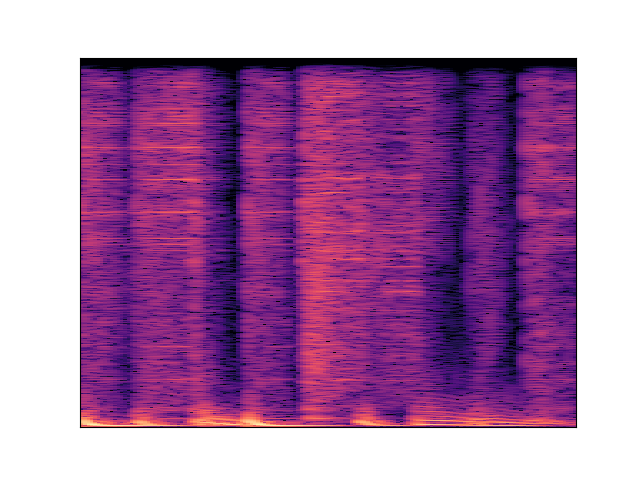
\includegraphics[width=\textwidth]{examples/original.wav.png}
\caption{Original}
\end{subfigure} \hfill

\begin{subfigure}[b]{0.2\textwidth}
\centering
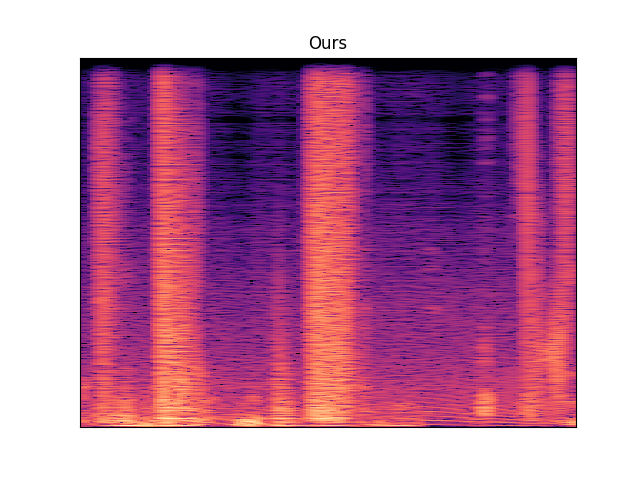
\includegraphics[width=\textwidth]{examples/temporal_audio_vae.wav.png}
\caption{Ours}
\end{subfigure} \hfill


\begin{subfigure}[b]{0.2\textwidth}
\centering
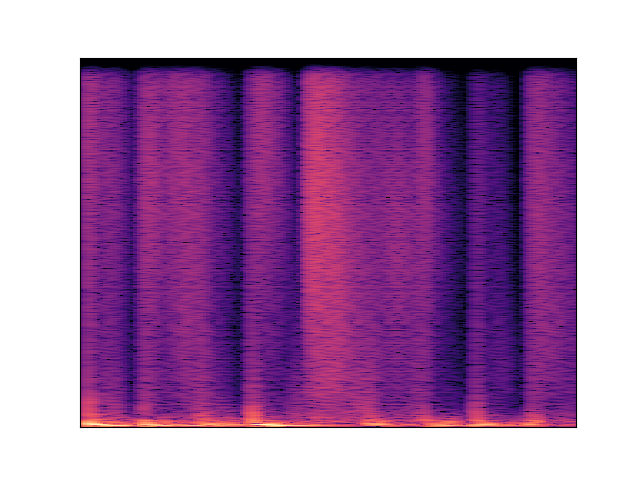
\includegraphics[width=\textwidth]{examples/rave_vae.wav.png}
\caption{Rave (}
\end{subfigure} \hfill

\begin{subfigure}[b]{0.2\textwidth}
\centering
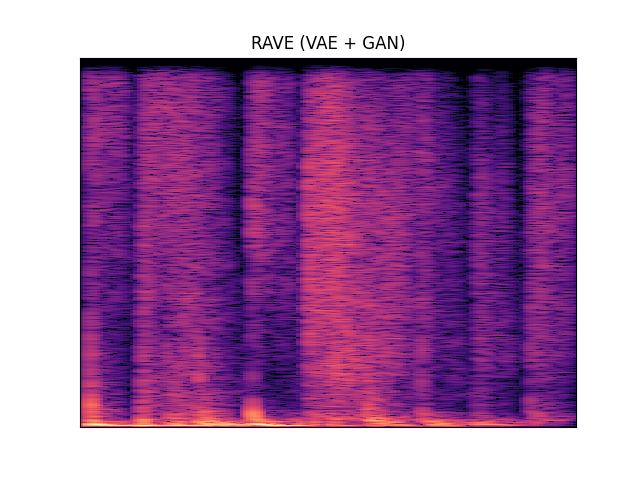
\includegraphics[width=\textwidth]{examples/rave.wav.png}
\caption{After}
\end{subfigure}

\caption[Hello]{Hello, this a minimal working example}
\end{figure}

% Unfortunately, this model and training scheme produces poor results: the reconstruction we obtain is far from the expected ground truth, and the generated sounds, if recognizable, are quite metallic and distorted in character.

% Some key points to address in order to achieve better reconstruction include the dimensions of the mel spectrogram, the depth of the encoder/decoder stack. The training procedure also sometimes showed numeric instability, resulting in NaN values creeping through and ultimately crashing the training, preventing us from training for a sufficient number of epochs.

\section{Realtime Audio Variational autoEncoder (RAVE)}

In order to highlight the characteristic information of the latent space, we can adapt the Realtime Audio Variational autoEncoder method \cite{caillonRAVEVariationalAutoencoder2021}. So, let us dig into the general procedure of this algorithm. 

When we code a VAE, the representation learned theoretically contains high-level features of the dataset. However, as we now want to deal with audio signals, we should consider a 
finer representation. Indeed, two similar signals can have slightly varying phases and result in totally different waveforms. Therefore, the reconstruction loss $\mathbb{E}_{q_\phi(\textbf{z} | \textbf{x}^{(i)})} [\log p_\theta(\textbf{x}^{(i)} | \textbf{z})]$ 
described above, if calculated from the raw waveform, penalizes the learned model because the phase variations are not included in the representation. This can corrupt the training process and induce low-level variations of the audio signal in the latent space, which are not relevant for sound rendering. To fix this, we can split the training process into two steps : representation learning and the adversarial fine-tuning.

So, the first step of the procedure is the representation learning. We will use the multiscale spectral distance $S$ described by Engel et al. \cite{engelDDSPDifferentiableDigital2020} in order to estimate the distance between the synthesized and real waveforms, defined by : 

\begin{equation} \label{spectral_dist}
    S(\textbf{x},\textbf{y}) = \sum_{n \in \mathcal{N}}\, \left[\, \frac{\lVert \text{STFT}_n(\textbf{x}) - \text{STFT}_n(\textbf{y}) \rVert_F}{\lVert \text{STFT}_n(\textbf{x}) \rVert_F} \,+\, \log (\lVert \text{STFT}_n(\textbf{x}) - \text{STFT}_n(\textbf{y}) \rVert_1)   \,\right],
\end{equation}

where $\mathcal{N}$ designates the set of scales, $\text{STFT}_n$ the amplitude of the short term Fourier transform with a window size n and hop size n/4, $\lVert \,.\, \rVert_F$ the Frobenius norm and $\lVert \,.\, \rVert_1$ the $l^1$ norm. We will therefore use an amplitude spectrum-based distance, which will take into account the phase reconstruction errors and contain the characteristic information of the signal.
We train the encoder and the decoder with the following loss :

\begin{equation}
    \mathcal{L}_{vae} (\textbf{x}) \,=\, \mathbb{E}_{\bm\hat{\textbf{x}} \sim p(\textbf{x}|\textbf{z})}[S(\textbf{x},\bm\hat {\textbf{x}})] \,+\, \beta . \mathcal{D}_{\text{KL}}(q_\phi (\textbf{z}|\textbf{x})||p(\textbf{z})).
\end{equation}

We train the model with this loss and once it converges, we move on to the next step.

The second step aims to improve the audio quality and its natural appearance. Once we assume that the learned representation reached a satisfactory state, we only train the decoder using an adversarial objective. The GANs are an implicit generative model which allows to sample from a complex distribution by changing it in a simplier one, called base distribution. We use here the latent space learned in the first step as base distribution and we train the decoder to produce synthetised signals similar to real signals, using a discriminator D. We use the hinge loss version of the GAN objective, defined as :



\begin{align}
    \mathcal{L}_{\text{dis}}(\textbf{x},\textbf{z}) &= \max(0, 1 - D(x)) + \mathbb{E}_{\bm\hat \textbf{x} \sim p(\textbf{x}|\textbf{z})}[\max(0, 1 + D(\bm\hat \textbf{x}))] \\
    \mathcal{L}_{\text{gen}}(\textbf{z}) &= -\mathbb{E}_{\bm\hat{ \textbf{x}} \sim p(\textbf{x}|\textbf{z})}[D(\bm\hat{ \textbf{x}})].
\end{align}

Since we do not want the synthetised signal $\bm\hat{\textbf{x}}$ to diverge too much from the real signal $\textbf{x}$, we keep minimizing the spectral distance defined above (\ref{spectral_dist}) by adding the feature matching loss $\mathcal{L}_{FM}$ \cite{kumarMelGANGenerativeAdversarial2019}. By combining everything, we end up at the wanted decoder :

\begin{equation}
    \mathcal{L}_{\text{total}} (\textbf{x},\textbf{z}) \,=\, \mathcal{L}_{\text{gen}}(\textbf{z})\,+\,\mathbb{E}_{\bm\hat{\textbf{x}} \sim p(\textbf{x}|\textbf{z})}[S(\textbf{x}, \bm\hat{\textbf{x}}) + \mathcal{L}_{\text{FM}}(\textbf{x}, \bm\hat{\textbf{x}})].
\end{equation}



Moreover, the loss we used in the first step consists of two terms : the  reconstruction term $\mathbb{E}_{\hat{\textbf{x}} \sim p(\textbf{x}|\textbf{z})}[S(\textbf{x},\bm\hat{ \textbf{x}})]$ and the regularisation term $\mathcal{D}_{\text{KL}}(q_\phi (\textbf{z}|\textbf{x})||p(\textbf{z}))$. The reconstruction aims to maximise the mutual information between the latent representation and the data distribution while the regularisation tends to make the posterior distribution independent from data. The final objective guides the model to acquire condensed representations of the data. In this process, meaningful latent factors exhibit the greatest KL divergence from the prior distribution, whereas less informative latent factors have a KL divergence approaching zero, as outlined by Higgins et al. \cite{higginsVVAELEARNINGBASIC2017}.

In order to better understand the latent representation, we will try to identify the most informative part of it. Our goal is to reduce the dimension of the representation learned to the minimum requierd to reconstruct the signal. To do this, we adapt the method for range and null space estimation to this problem.

Let $\textbf{Z} \in \mathbb{R}^{b \times d}$ a matrix composed of $b$ samples $\textbf{z} \in \mathbb{R}^d$, where $\textbf{z} \sim q_\phi(\textbf{z}|\textbf{x})$. Since the collapsed parts of \textbf{Z} has a high variance, we first start to subtract the variance from \textbf{Z} by considering the matrix $\textbf{Z}' \in \mathbb{R}^{b \times d}$ :
\begin{equation}
    \textbf{Z}_i' = \text{argmax}_{\textbf{z}} q_\phi (\textbf{z}|\textbf{x}).
\end{equation}
Thus, the dimensions of the posterior distribution \(q_{\phi}(\textbf{z}|\textbf{x})\) that have collapsed to the prior \(p(\textbf{z})\) will yield a constant value in \(\textbf{Z}'\). To address this, we nullify this constant value by subtracting the mean of \(\textbf{Z}'\) along the first dimension. The only dimension of $\textbf{Z}'$ with values different from zero will be correlated to the input, which contais the informative part of the latent space.

We can now decompose this centerd matrix into singular values :
\begin{equation}
    \textbf{Z}'\,=\, \textbf{U}\, \bm\Sigma \,^{\textbf{t}}\textbf{V},
\end{equation}

where $\bm\Sigma$ is composed by the singular values of $\textbf{Z}'$.
Then, it can be showed that the rank $r$ of $\textbf{Z}'$ is equal to the number of non-zero singular values of $\textbf{Z}'$ present in $\bm\Sigma$. But the singular values that we want to identify as zero are not very likely to be strictly equal to zero, given the high variabilities in real data. So, if we want to find the rank of $\textbf{Z}'$, we must define a fidelity parameter $f \in [0,1]$ and the associated rank $r_f$ defined as the the smallest integer verifying :
\begin{equation}
    \frac{\sum_{i \leq r_f} \bm\Sigma_{ii}}{\sum_i \bm\Sigma_{ii}} \geq f.
\end{equation}

for a specific value of $f$ and a latent representation $\textbf{z} \sim q_\phi (\textbf{z}|\textbf{x})$, we can reduce the dimension of $\textbf{z}$ by projecting it on the base defined by $^\textbf{t}\textbf{V}$. We then only keep the $r_f$ first dimensions to obtain a low-rank representation of $\textbf{z}_f$. Note that this dimension depends on $f$ and the dataset. Finally, we concatenate $\textbf{z}_f$ with a noise sampled from the prior distribution, we reproject it on the the original basis using $\textbf{V}$ and we give it to the decoder.

%\section{Citations, figures, tables}
%\label{others}
% \end{comment}
\begin{comment}
    

    These instructions apply to everyone.
    
    
    \subsection{Citations within the text}
    
    
    The \verb+natbib+ package will be loaded for you by default.  Citations may be
    author/year or numeric, as long as you maintain internal consistency.  As to the
    format of the references themselves, any style is acceptable as long as it is
    used consistently.
    
    
    The documentation for \verb+natbib+ may be found at
    \begin{center}
      \url{http://mirrors.ctan.org/macros/latex/contrib/natbib/natnotes.pdf}
    \end{center}
    Of note is the command \verb+\citet+, which produces citations appropriate for
    use in inline text.  For example,
    \begin{verbatim}
       \citet{hasselmo} investigated\dots
    \end{verbatim}
    produces
    \begin{quote}
      Hasselmo, et al.\ (1995) investigated\dots
    \end{quote}
    
    
    If you wish to load the \verb+natbib+ package with options, you may add the
    following before loading the \verb+neurips_2023+ package:
    \begin{verbatim}
       \PassOptionsToPackage{options}{natbib}
    \end{verbatim}
    
    
    If \verb+natbib+ clashes with another package you load, you can add the optional
    argument \verb+nonatbib+ when loading the style file:
    \begin{verbatim}
       \usepackage[nonatbib]{neurips_2023}
    \end{verbatim}
    
    
    As submission is double blind, refer to your own published work in the third
    person. That is, use ``In the previous work of Jones et al.\ [4],'' not ``In our
    previous work [4].'' If you cite your other papers that are not widely available
    (e.g., a journal paper under review), use anonymous author names in the
    citation, e.g., an author of the form ``A.\ Anonymous'' and include a copy of the anonymized paper in the supplementary material.
    
    
    \subsection{Footnotes}
    
    
    Footnotes should be used sparingly.  If you do require a footnote, indicate
    footnotes with a number\footnote{Sample of the first footnote.} in the
    text. Place the footnotes at the bottom of the page on which they appear.
    Precede the footnote with a horizontal rule of 2~inches (12~picas).
    
    
    Note that footnotes are properly typeset \emph{after} punctuation
    marks.\footnote{As in this example.}
    
    
    \subsection{Figures}
    
    
    \begin{figure}
      \centering
      \fbox{\rule[-.5cm]{0cm}{4cm} \rule[-.5cm]{4cm}{0cm}}
      \caption{Sample figure caption.}
    \end{figure}
    
    
    All artwork must be neat, clean, and legible. Lines should be dark enough for
    purposes of reproduction. The figure number and caption always appear after the
    figure. Place one line space before the figure caption and one line space after
    the figure. The figure caption should be lower case (except for first word and
    proper nouns); figures are numbered consecutively.
    
    
    You may use color figures.  However, it is best for the figure captions and the
    paper body to be legible if the paper is printed in either black/white or in
    color.
    
    
    \subsection{Tables}
    
    
    All tables must be centered, neat, clean and legible.  The table number and
    title always appear before the table.  See Table~\ref{sample-table}.
    
    
    Place one line space before the table title, one line space after the
    table title, and one line space after the table. The table title must
    be lower case (except for first word and proper nouns); tables are
    numbered consecutively.
    
    
    Note that publication-quality tables \emph{do not contain vertical rules.} We
    strongly suggest the use of the \verb+booktabs+ package, which allows for
    typesetting high-quality, professional tables:
    \begin{center}
      \url{https://www.ctan.org/pkg/booktabs}
    \end{center}
    This package was used to typeset Table~\ref{sample-table}.
    
    
    \begin{table}
      \caption{Sample table title}
      \label{sample-table}
      \centering
      \begin{tabular}{lll}
        \toprule
        \multicolumn{2}{c}{Part}                   \\
        \cmidrule(r){1-2}
        Name     & Description     & Size ($\mu$m) \\
        \midrule
        Dendrite & Input terminal  & $\sim$100     \\
        Axon     & Output terminal & $\sim$10      \\
        Soma     & Cell body       & up to $10^6$  \\
        \bottomrule
      \end{tabular}
    \end{table}
    
    \subsection{Math}
    Note that display math in bare TeX commands will not create correct line numbers for submission. Please use LaTeX (or AMSTeX) commands for unnumbered display math. (You really shouldn't be using \$\$ anyway; see \url{https://tex.stackexchange.com/questions/503/why-is-preferable-to} and \url{https://tex.stackexchange.com/questions/40492/what-are-the-differences-between-align-equation-and-displaymath} for more information.)
    
    \subsection{Final instructions}
    
    Do not change any aspects of the formatting parameters in the style files.  In
    particular, do not modify the width or length of the rectangle the text should
    fit into, and do not change font sizes (except perhaps in the
    \textbf{References} section; see below). Please note that pages should be
    numbered.
\end{comment}

\printbibliography
% \bibliography



\section{Appendixes}


\subsection{RAVE architecture}

\subsection{Task distribution}

% TODO remplir

\begin{itemize}
    \item[•] Paul
    \begin{itemize}
        \item[$\circ$] 
        \item[$\circ$] 
        \item[$\circ$] 
    \end{itemize}
    \item[•] Antoine
    \begin{itemize}
        \item[$\circ$] 
        \item[$\circ$] 
        \item[$\circ$] 
    \end{itemize}
    \item[•] Etienne
    \begin{itemize}
        \item[$\circ$] 
        \item[$\circ$] 
        \item[$\circ$] 
    \end{itemize}
    \item[•] Enguérand
    \begin{itemize}
        \item[$\circ$] 
        \item[$\circ$] 
        \item[$\circ$] 
    \end{itemize}



\end{itemize}

% \section*{References}



% [1] Antoine Caillon and Philippe Esling.  Rave: A variational autoencoder for fast and high-quality neural audio synthesis. \textit{arXiv preprint arXiv:2111.05011}, 2021.


% [2] Esse Engel, Kumar Krishna Agrawal, Shuo Chen, Ishaan Gulrajani, Chris Donahue and Adam Roberts. Gan- synth: Adversarial neural audio synthesis. \textit{arXiv preprint arXiv:1902.08710}, 2019.


% [3] Jesse Engel, Lamtharn Hantrakul, Chenjie Gu and Adam Roberts. Ddsp: Differentiable digital signal processing. \textit{arXiv preprint arXiv:2001.04643}, 2020.

% [4] Irina Higgins, Loïc Matthey, Arka Pal, Christopher Burgess, Xavier Glorot, Matthew M Botvinick, Shakir Mohamed, and Alexander Lerchner. beta-vae: Learning basic visual concepts with a constrained variational frame- work. \textit{In ICLR}, 2017.


% [5] Diederik P Kingma and Max Welling. Auto-encoding variational bayes. \textit{arXiv:1312.6114}, 2013. 



% [6] Kundan Kumar, Rithesh Kumar, Thibault de Boissiere, Lucas Gestin, Wei Zhen Teoh, Jose Sotelo, Alexandre de Brebisson, Yoshua Bengio, and Aaron Courville. MelGAN: Generative Adversarial Networks for Conditional Waveform Synthesis. \textit{arXiv, 10 2019}.



%%%%%%%%%%%%%%%%%%%%%%%%%%%%%%%%%%%%%%%%%%%%%%%%%%%%%%%%%%%%


\end{document}